% https://www.latex4technics.com/?note=U130YI
% https://tex.stackexchange.com/a/370552/173708
\documentclass[a4paper, 12pt]{article}
\usepackage[paperwidth=5in, paperheight=3.2in]{geometry}
\usepackage{pgfplots}
\pgfplotsset{compat=newest}
\geometry{left=0mm, right=3mm,top=6mm, bottom=3mm,}

\definecolor{mygr}{HTML}{e6e6e6}

\begin{document}
\begin{figure}[!t]
  \centering
  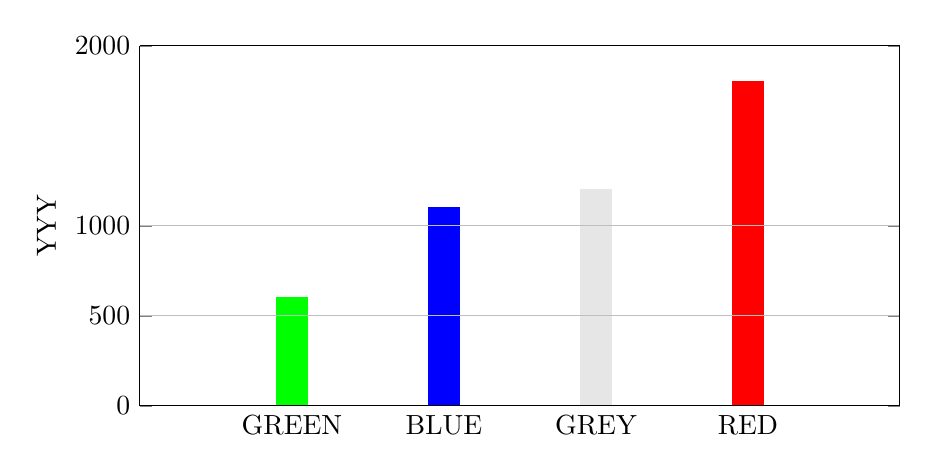
\begin{tikzpicture}
    \begin{axis}[
        /pgf/number format/1000 sep={},
        width=3.8in,
        height=1.8in,
        at={(0.758in,0.981in)},
        scale only axis,
        clip=false,
        separate axis lines,
        axis on top,
        xmin=0,
        xmax=5,
        xtick={1,2,3,4},
        x tick style={draw=none},
        xticklabels={GREEN,BLUE,GREY,RED},
        ytick={0, 500, 1000, 2000},
        ymin=0,
        ymax=2000,
        ylabel={YYY},
        ymajorgrids,
        every axis plot/.append style={
          ybar,
          bar width=.2,
          bar shift=0pt,
          fill
        }
      ]
      \addplot[green]coordinates {(1,600)};
      \addplot[blue]coordinates{(2,1100)};
      \addplot[mygr]coordinates{(3,1200)};
      \addplot[red]coordinates{(4,1800)};
    \end{axis}
  \end{tikzpicture}
\end{figure}
\end{document}
